\documentclass{article}

% Language setting
% Replace `english' with e.g. `spanish' to change the document language
\usepackage[english]{babel}

% Set page size and margins
% Replace `letterpaper' with `a4paper' for UK/EU standard size
\usepackage[letterpaper,top=2cm,bottom=2cm,left=3cm,right=3cm,marginparwidth=1.75cm]{geometry}

% Useful packages
\usepackage{amsmath}
\usepackage{graphicx}
\usepackage[colorlinks=true, allcolors=blue]{hyperref}

\title{Problem Set 6}
\author{Justin Canova}

\begin{document}
\maketitle

\section{Introduction}

The following interaction plots are meant to convey the following OLS regression using z-scored values.

\begin{equation}
    Future_{aspirations} = \beta_0 + \beta_1 \text{Self\_Rank}_i + \beta_2 \text{Yrs\_reffing}_i + \beta_3 \text{W\_Income}_i + \beta_4 \text{Age}_i + \beta_5 \text{Kids}_i + \beta_6 \text{Educ}_i 
\end{equation}

\begin{equation}
    + \beta_7 \text{Current}_i + \beta_8 \text{Gender}_i + \beta_9 (\text{Yrs\_reffing}_i \times \text{Self\_Rank}_i) + \varepsilon_i
\end{equation}

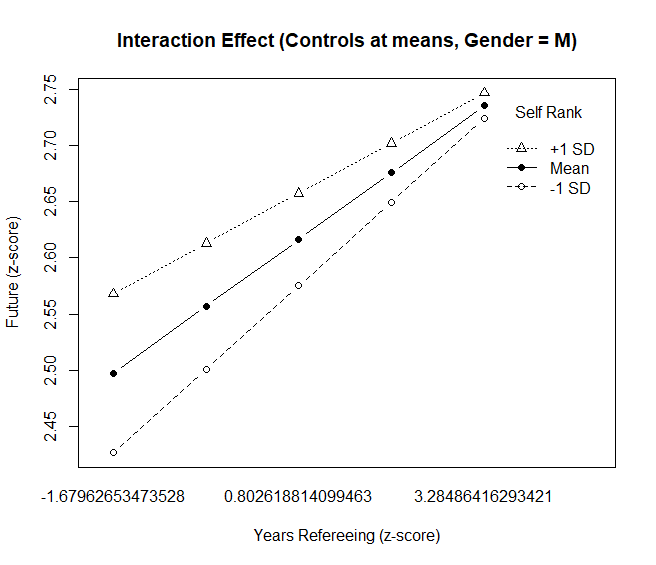
\includegraphics[]{PS6a_Canova.png}
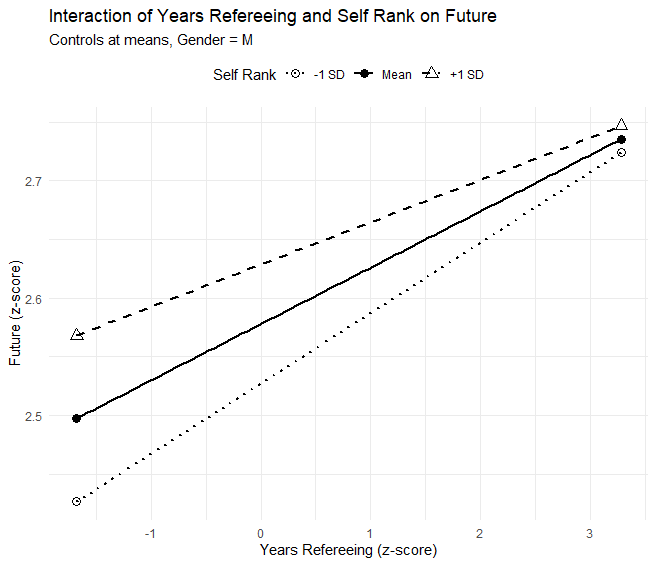
\includegraphics[]{PS6b_Canova.png}
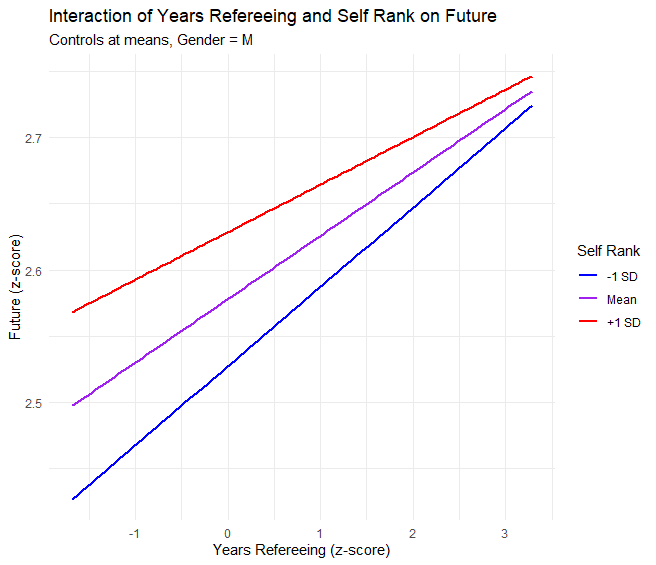
\includegraphics[]{PS6c_Canova.png}

\end{document}